\section{Redex: a Domain-Specific Language for Semantics}

Redex is a scripting language and set of associated tools supporting
the conception, design, construction, and testing of semantic systems
such as programming languages, type systems, program logics, and
program analyses. As a scripting language, it enables an engineer to
create executable specifications of common semantic elements such as
grammars, reduction relations, judgments, and metafunctions; the basic
elements of formal systems. It includes a number of software
engineering inspired features to make models robust and includes tools
for typesetting mod- els and generating algebraic steppers for
exploring program behaviors. In brief, Redex supports all phases of
the semantic engineering life-cycle.

\subsection{Racket: a General-Purpose Host Language}

Redex is a domain-specific language (DSL) embeded within the
general-purpose language Racket.  Racket is a descendant of Lisp and
adopts much of Lisp's fully parenthesized prefix notation.  It comes
with an interactive development environment, called DrRacket, and has
a large corpus of libraries.  It has been developed over the last
twenty or so years by the PLT research group, which is distributed
across several different universities in the USA.  The group has
developed Racket in part to support their educational work and in part
as a vehicle for researching programming languages.  

The basic unit of code in Racket is a module, which must first declare
which language it is written in with the {\tt \#lang} directive:
\begin{verbatim}
#lang racket
\end{verbatim}
It turns out Racket is more than just a single programming language
but a ecosystem of many different languages than can interoperate.
The {\tt racket} language is the core language of the system, but
there are many others, such as a typed variant of {\tt racket} called
{\tt typed/racket}, Datalog, Algol 60, a documentation language called
{\tt scribble}, and many more.  We will only be concerned with a very
small subset of {\tt racket}, though.

After the language declaration, a module may declare what it requires
and provides, followed by a series of definitions or expressions.
For example, this module defines and then uses the factorial function:
\begin{verbatim}
#lang racket
(define (fact n)
  (if (zero? n)
      1
      (* n (fact (sub1 n)))))

(fact 5)
\end{verbatim}

When run inside DrRacket (by pressing the ``Run'' button), the window
is split into two parts: the definitions area, which contains the
source code of the module, and the interactions area, which can be
used to interact with the program above.  An example is shown in
figure~\ref{fig:drracket}.
\begin{figure}
\begin{center}
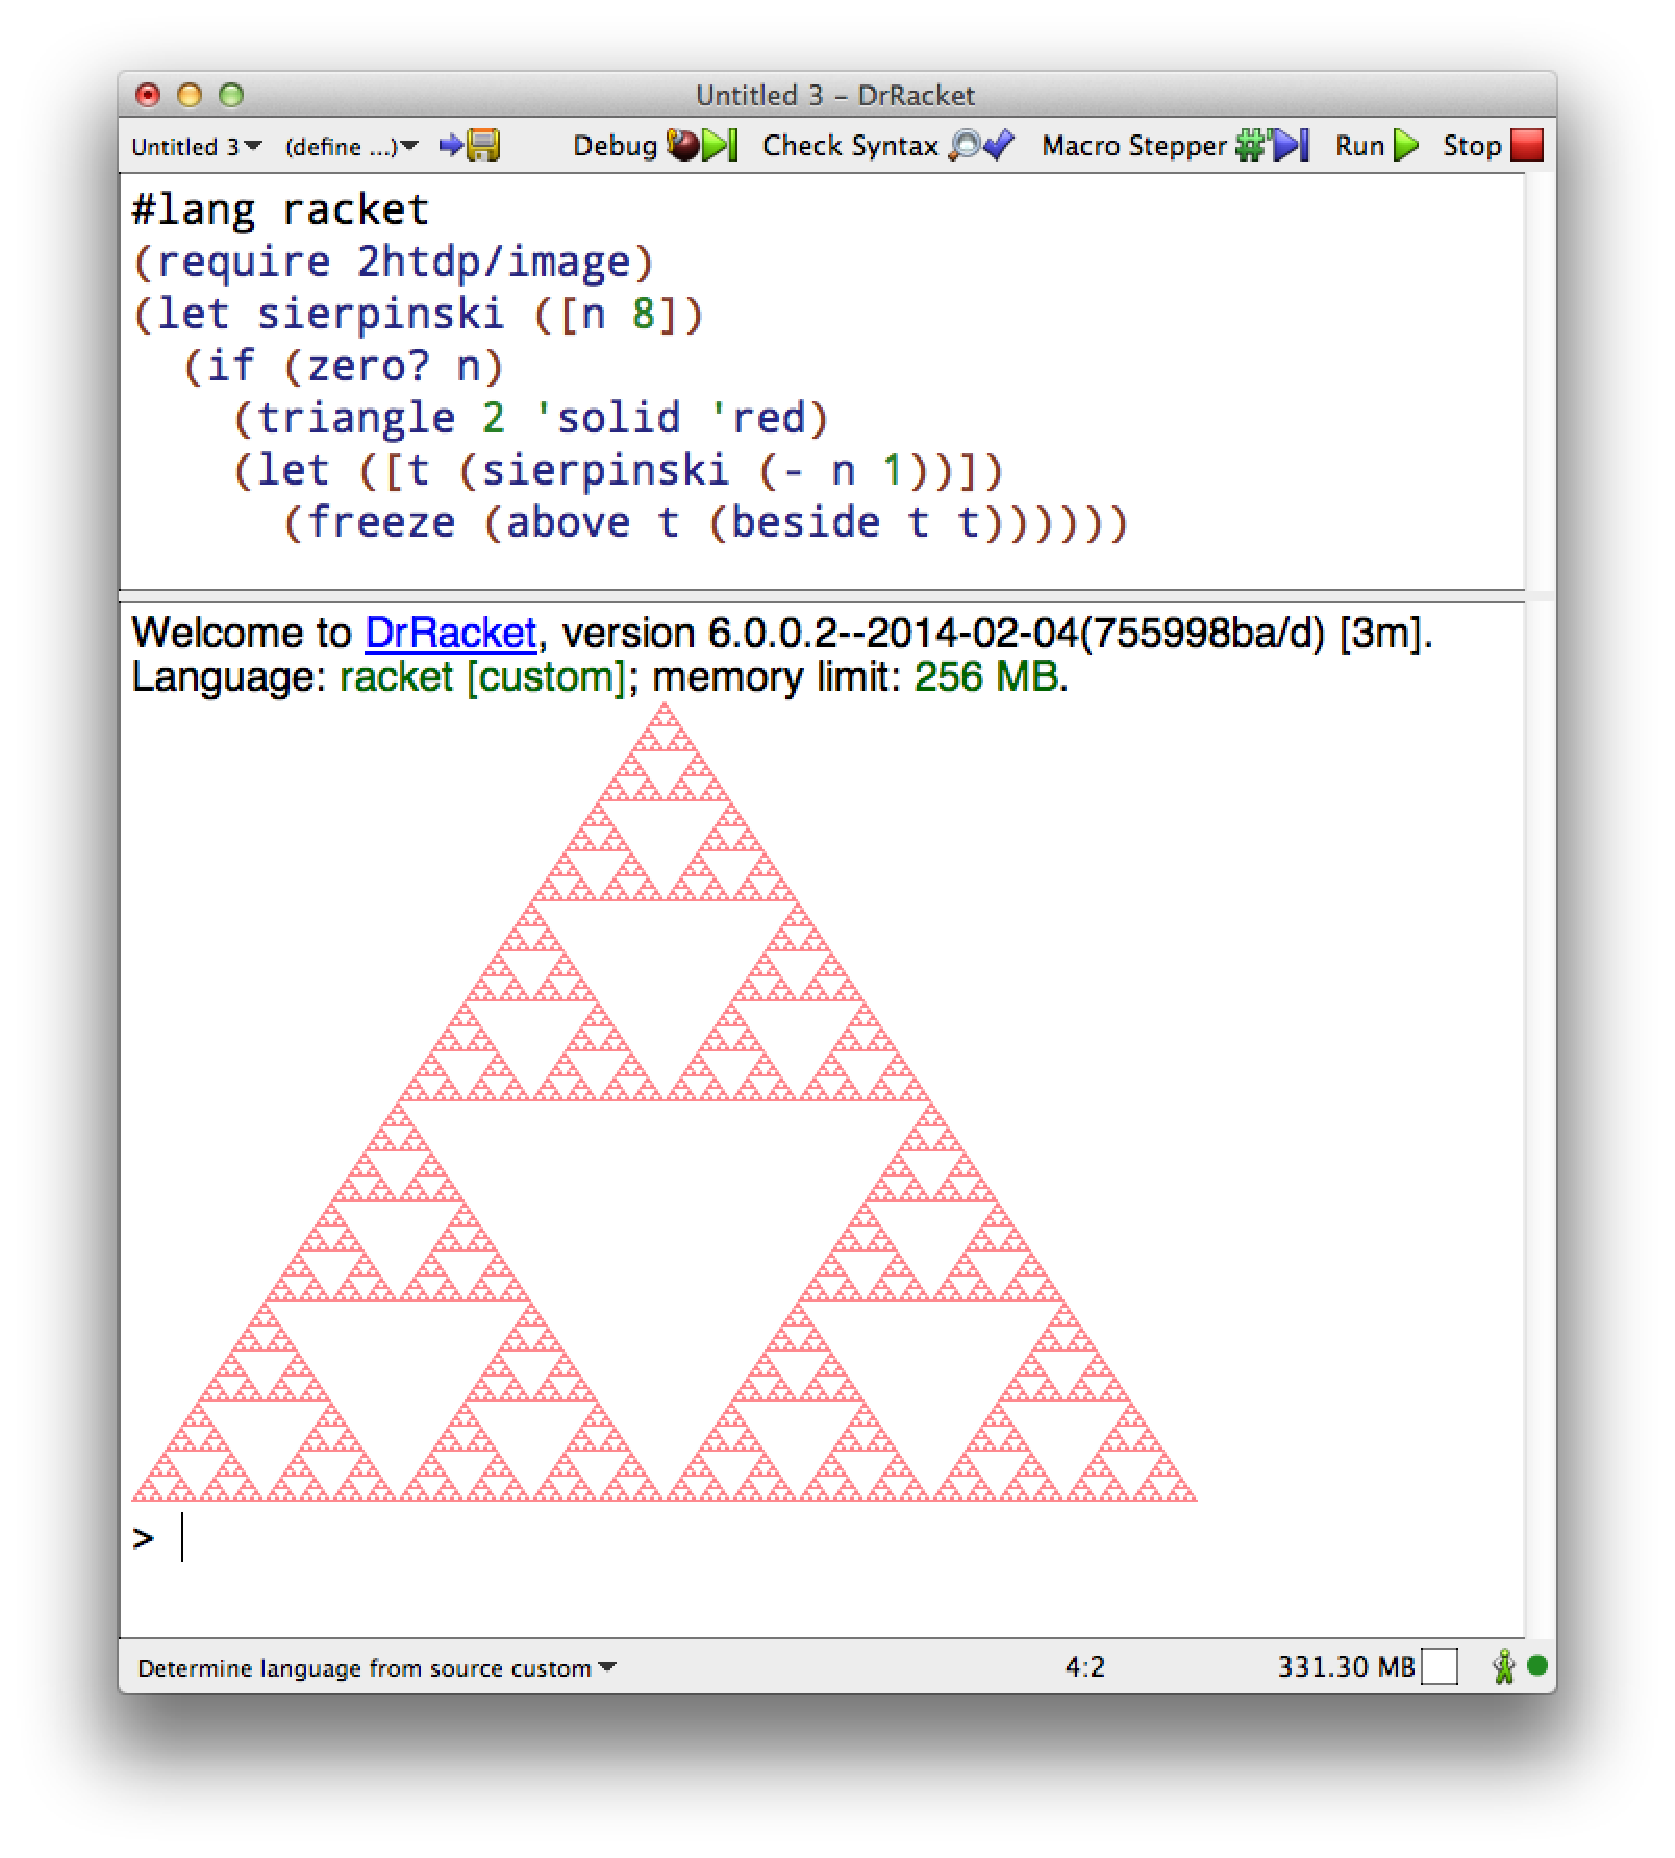
\includegraphics[width=5in]{figs/drracket}
\end{center}
\caption{The DrRacket interactive development environment.}
\label{fig:drracket}
\end{figure}


The interactions area has a prompt for accepting expressions to
evaluate.  Any definitions from the module are avaiable within the
interactions window, so we can experiment and calculate other results
of factorial:
\begin{verbatim}
> (fact (fact 5))
6689502913449127057588118054090372586752746333138029
8102956713523016335572449629893668741652719849813081
5763789321409055253440858940812185989848111438965000
5964960521256960000000000000000000000000000
\end{verbatim}

Changes that are made to the module are not immediately reflected in
the interactions window.  The program has to be re-run, which creates
a fresh interactions window, discarding anything you may have entered.
(But scrolling through a history of expressions is possible with
Cmd+Up.)


%% Because of this, the language incorporates an array of cutting edge PL
%% features for creating programming languages.  In fact, ``Racket'' is
%% not really a programming language, but a programming language
%% ecosystem.  Modules, which are the basic unit of code, can be written
%% in any of dozens of various languages

\subsection{Defining a Language}

To construct a Redex model of a language, the first thing to do is
declare the host language ({\tt racket}) and require the Redex
library:
\begin{verbatim}
#lang racket
(require redex)
\end{verbatim}

Defining the syntax of a language is accomplished with {\tt
  define-language}, which gives the grammar of terms for the language:
\begin{verbatim}
(define-language A
  (e ::= 
     v
     (Pred e)
     (Succ e)
     (Plus e e)
     (Mult e e))
  (v ::= i)
  (i j k ::= integer))
\end{verbatim}
This establishes the set of terms in the language {\tt A}, and also
establishes a number of meta-variable names which can be used to
pattern match terms.

For example, we can query the language to see if the term {\tt 4} is
in the set of values ranged over by meta-variable {\tt e}:
\begin{verbatim}
> (redex-match? A e (term 4))
#t
\end{verbatim}
It's also true that {\tt i} ranges over {\tt 4}:
\begin{verbatim}
> (redex-match? A i (term 4))
#t
\end{verbatim}
But while {\tt (Pred 4)} is in {\tt e}, it is not in {\tt i}:
\begin{verbatim}
> (redex-match? A e (term (Pred 4)))
#t
> (redex-match? A i (term (Pred 4)))
#f
\end{verbatim}

\subsection{Terms}

Terms in Redex are constructed with the {\tt term} form.  To a first
approximation, {\tt term} is just a synonym for {\tt quote}, which
constructs literal data.  In fact we could have constructed our
examples in the previous section with {\tt quote}, which can be written
{\tt (quote e)} or {\tt 'e} for short:
\begin{verbatim}
> (redex-match? A e '(Pred 4))
#t
> (redex-match? A i '(Pred 4))
#f
\end{verbatim}

The difference between {\tt term} and {\tt quote} is that {\tt term}
interprets some of the literal data.  The simplest example of this is
that {\tt term} interprets occurrences of bound meta-variables and
substitutes their values for the occurrences.  For example, we can
define a term variable with {\tt define-term} and then refer to it
within {\tt term} expressions:
\begin{verbatim}
> (define-term five 5)
> (term five)
5
> (quote five)
'five
\end{verbatim}
As we'll see, Redex comes with a powerful pattern matcher that let's
us match terms against term patterns and bind variables for use within
terms.

Another feature of {\tt term} is that it is possible to escape out of
the term language and back in to Racket.  This is accomplished with
{\tt unquote}.  The notation {\tt ,e} is a Racket shorthand for {\tt
  (unquote e)} and it signals to Redex not to interpret {\tt e} as a
term, but rather as a Racket expression which evaluates to a term.  In
other words.  Using the {\tt term} constructor within the expression
re-enters the Redex world, and this nesting can be arbitrarily deep.
Here are some examples:
\begin{verbatim}
> (term (Plus (add1 5)))
'(Plus (add1 5))
> (term (Plus ,(add1 5)))
'(Plus 6)
> (term (Plus ,(add1 (term five))))
'(Plus 6)
\end{verbatim}


\subsection{Defining a Reduction Relation}

A reduction relation is a value in Redex, constructed with the {\tt
  reduction-relation} form.  Defining the $\areducename$ relation is
achieved with:
\begin{verbatim}
(define a
  (reduction-relation
   A
   (--> (Pred i) ,(sub1 (term i)) pred)
   (--> (Succ i) ,(add1 (term i)) succ)
   (--> (Plus i j) ,(+ (term i) (term j)) plus)
   (--> (Mult i j) ,(* (term i) (term j)) mult)))
\end{verbatim}
A {\tt reduction-relation} specifies which language it operates on, in
this case {\tt A}.  The language determines the interpretation of the
meta-variables (and what whether a peice of syntax is a
meta-variable).  The relation is written as a set of axioms, each of
which has the form {\tt (--> $L\;R\;\mathit{name}$)} where $L$ is a
\deftech{pattern} and $R$ is a \deftech{template} and $\mathit{name}$
is an optional name for the rule.  Applying a reduction relation to a
term matches the term against each pattern and if the match is
succesful produces the template with each meta-variable replaced by
the corresponding substructure of the pattern match.

A reduction relation can be applied with {\tt apply-reduction-relation}:
\begin{verbatim}
> (apply-reduction-relation a (term (Pred 5)))
'(4)
\end{verbatim}
When the relation is not defined on a term, the empty list is produced:
\begin{verbatim}
> (apply-reduction-relation a (term (Mult (Pred 4) 5)))
'()
\end{verbatim}

There are a few operations on reduction relations that produce new
reduction relations.  For example, {\tt compatible-closure} computes
the compatible closure of a relation:
\begin{verbatim}
> (apply-reduction-relation (compatible-closure a A e)
                            (term (Mult (Pred 4) 5)))
'((Mult 3 5))
\end{verbatim}
Like any value, we can name this relation using {\tt define}:
\begin{verbatim}
(define ->a (compatible-closure a A e))
\end{verbatim}
The {\tt apply-reduction-relation*} function computes the set of
irreducible terms that are in the transitive closure of a given
relation:
\begin{verbatim}
> (apply-reduction-relation* ->a (term (Mult (Pred 4) 5)))
'(15)
\end{verbatim}

The {\tt traces} function will visualize the reduction semantics as a
graph of related terms.  For example,
\begin{verbatim}
> (traces ->a (term (Mult (Plus (Succ 2) (Mult 2 2)) (Plus 5 5))))
\end{verbatim}
will launch a window displaying the graph in figure~\ref{fig:graph}.
\begin{figure}
\begin{center}
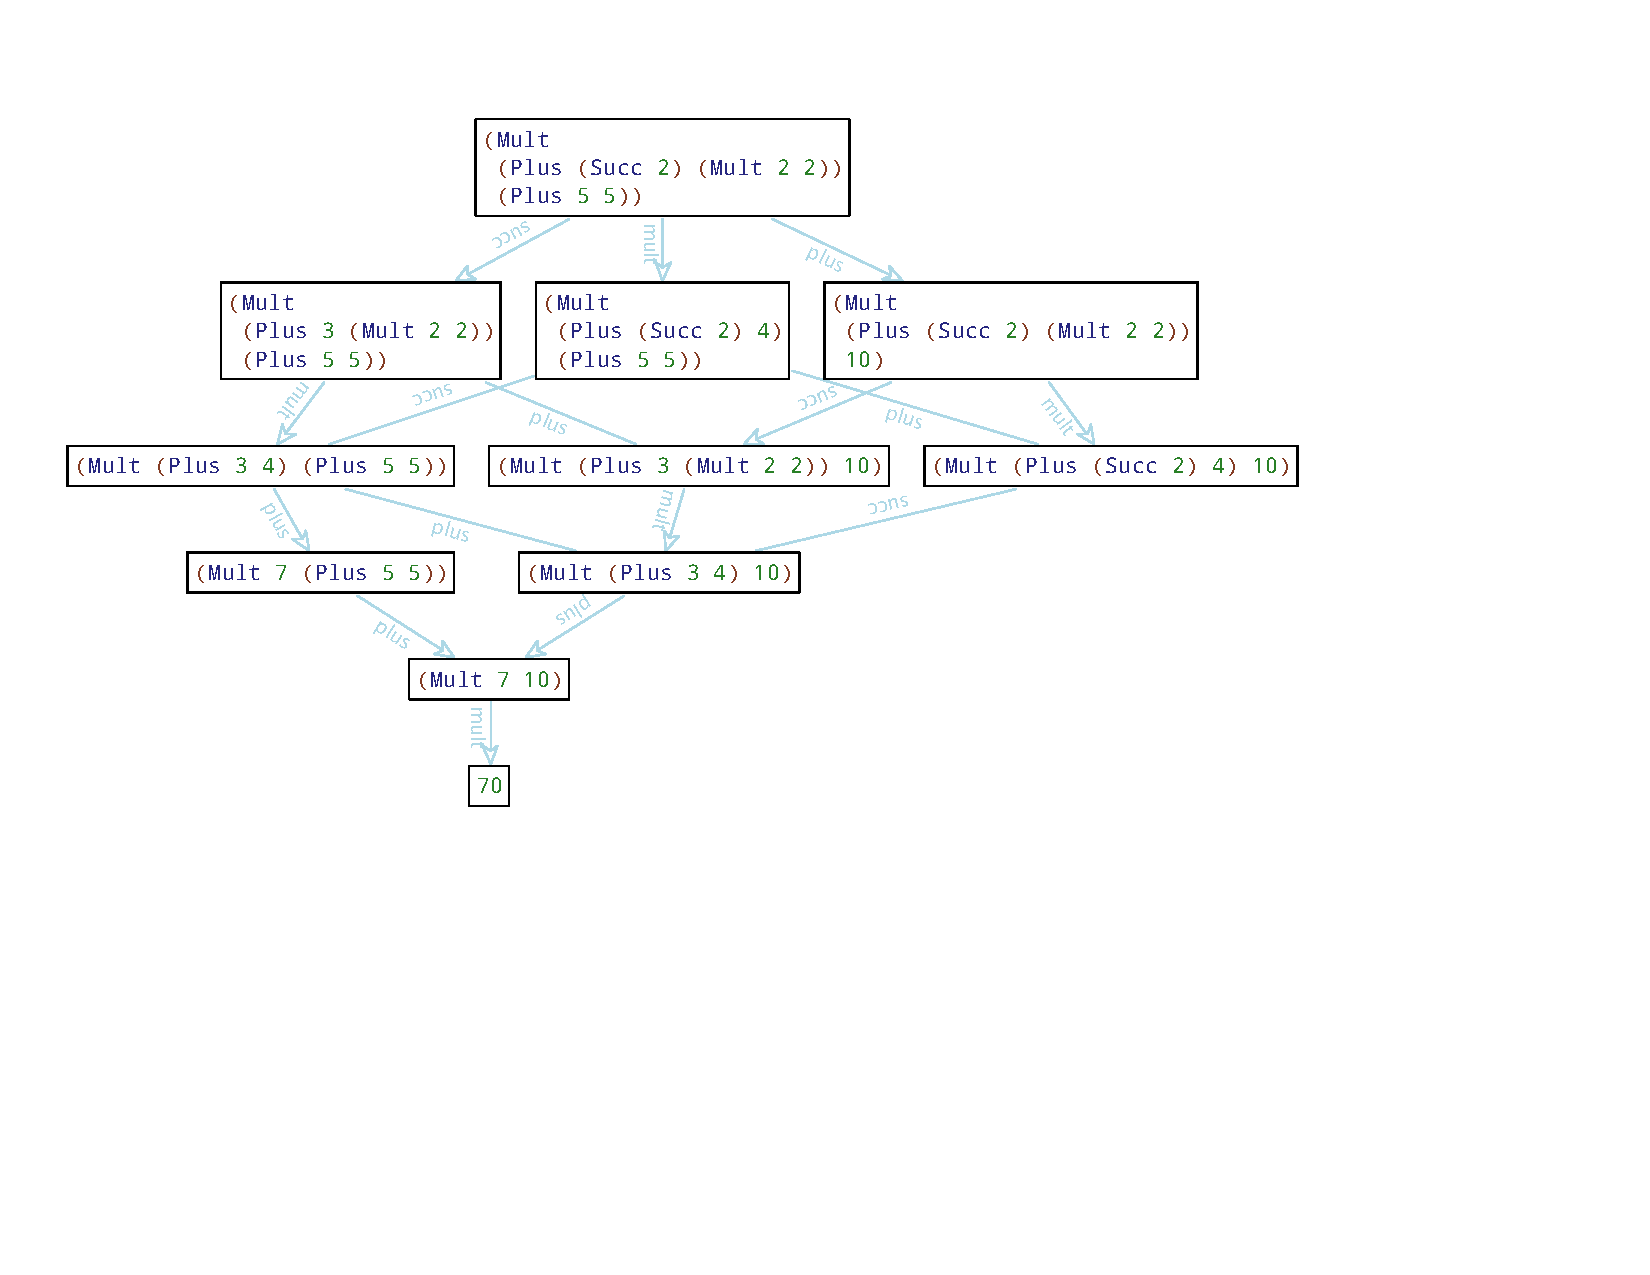
\includegraphics[width=5in]{figs/reduction-graph.pdf}
\end{center}
\caption{Example reduction graph.}
\label{fig:graph}
\end{figure}


\subsection{Defining metafunctions}

A metafunction is a function that is interpreted within the term
language.  Here is the natural semantics function written as a
metafunction in Redex:
\begin{verbatim}
(define-metafunction A
  [(eval v) v]
  [(eval (Pred e)) ,(sub1 (term (eval e)))]
  [(eval (Succ e)) ,(add1 (term (eval e)))]  
  [(eval (Plus e_1 e_2)) 
   ,(+ (term (eval e_1))
       (term (eval e_2)))]
  [(eval (Mult e_1 e_2))
   ,(* (term (eval e_1))
       (term (eval e_2)))])
\end{verbatim}

The function is defined by a series of pattern and template clauses,
much like a reduction relation but without the {\tt -->} notation.
Unlike a reduction relation, the patterns are tried in order and the
result of the metafunction application is the instantiated template of
the first matching clause.  An error is signalled if no clause
matches.

Once a metafunction is defined, it is applied whenever it occurs with
a {\tt term}:
\begin{verbatim}
> (term (eval (Mult (Pred 5) (Succ 8))))
36
> (term (Mult (Pred 5) (eval (Succ 8))))
'(Mult (Pred 5) 9)
\end{verbatim}

It's important to notice that this defines a \emph{function}, not a
\emph{relation}.  Since we know that $\Downarrow$ for $\Arith$ is a
function, this is a correct model of $\Downarrow$, but it would not be
if $\Downarrow$ were realy a relation, such as with the natural
semantics of imprecise errors for $\Barith$.  To model relations (that
are not reduction relations), we need another mecahnism: {\tt
  define-judgment-form}.

\subsection{Contexts}

Evaluation contexts can also be specified as part of a language's
grammar.  We can add the following to the {\tt define-language} for
{\tt A}:
\begin{verbatim}
  (E ::=
     hole
     (Pred E)
     (Succ E)
     (Mult E e)
     (Mult v E)
     (Plus E e)
     (Plus v E))
\end{verbatim}

Within a reduction relation and other patterns, {\tt in-hole} can be
used to match terms within a context.  For example, the standard
reduction relation can be defined as:
\begin{verbatim}
(define -->a
  (reduction-relation
   A
   (--> (in-hole E (Pred i)) (in-hole E ,(sub1 (term i))))
   (--> (in-hole E (Succ i)) (in-hole E ,(add1 (term i))))
   (--> (in-hole E (Mult i j)) (in-hole E ,(* (term i) (term j))))
   (--> (in-hole E (Plus i j)) (in-hole E ,(+ (term i) (term j))))))
\end{verbatim}

Since each of these rules has a repeated structure of using {\tt
  in-hole}, it's possible to define a shortcut:
\begin{verbatim}
(define -->a
  (reduction-relation
   A
   (~~> (Pred i) ,(sub1 (term i)))                                                              
   (~~> (Succ i) ,(add1 (term i)))                                                                   
   (~~> (Mult i j) ,(* (term i) (term j)))
   (~~> (Plus i j) ,(+ (term i) (term j)))
   with
   [(--> (in-hole E e_1) (in-hole E e_2))
    (~~> e_1 e_2)]))
\end{verbatim}
Or, we could simple compute the relation by using {\tt
  context-closure} and the existing reduction relation {\tt a}:
\begin{verbatim}
(define -->a
  (context-closure a A E))
\end{verbatim}

\subsection{Defining a Judgment (Relation)}

Defining a relation is accomplished with the {\tt
  define-judgment-form} notation:
\begin{verbatim}
(define-judgment-form A
  #:mode (evalr I O)
  [(evalr v v)]
  [(evalr e v)
   -----------
   (evalr (Pred e) ,(sub1 (term v)))]
  [(evalr e v)
   -----------
   (evalr (Succ e) ,(add1 (term v)))]  
  [(evalr e_1 v_1)
   (evalr e_2 v_2)
   ---------------
   (evalr (Plus e_1 e_2) ,(+ (term v_1) (term v_2)))]
  [(evalr e_1 v_1)
   (evalr e_2 v_2)
   ---------------
   (evalr (Mult e_1 e_2) ,(* (term v_1) (term v_2)))])
\end{verbatim}

A judgment is a relation that is being modelled computationally as a
function.  The {\tt \#:mode} keyword gives a mode specification which
declares which parts of the relation can be consider inputs ({\tt I})
and which parts can be considered outouts ({\tt O}), which can be
thought of as specifying which positions are inputs and outputs in
this function.

A judgment is used with {\tt judgment-holds} form.  It can be used in
two ways, the first is to check if the relation holds on particular
values.  So for example, we can check that {\tt (Succ (Succ 4))}
evaluates to {\tt 6} with:
\begin{verbatim}
> (judgment-holds (evalr (Succ (Succ 4)) 6))
#t
\end{verbatim}
It's also possible to compute the set of all values related to {\tt
  (Succ (Succ 4))} with:
\begin{verbatim}
> (judgment-holds (evalr (Succ (Succ 4)) v) v)
'(6)
\end{verbatim}
The set of related terms is given as a list of results (in case, it's
always a singleton list).

\subsection{Property-Based Testing}

Semantic models are often buggy, just like programs.  One of the
easiest and quickest ways to test code is to state properties you
believe to be true and then test that the property holds for a bunch
of random inputs.

We believe the standard reductions semantics and natural semantics
correspond in the following way, for all {\tt e}:
\begin{verbatim}
  (equal? (apply-reduction-relation* -->a (term e))
          (judgment-holds (evalr e v) v))
\end{verbatim}
That is, for any term, the set of irreducible values reached by
iterating the standard reduction relation are exactly equal to the set
of values related by the natural semantics relation.  Redex will
generate random expressions and search for a counterexample with {\tt
  redex-check}:
\begin{verbatim}                                                                          
> (redex-check A e
               (equal? (apply-reduction-relation* -->a (term e))
                       (judgment-holds (evalr e v) v)))
redex-check: no counterexamples in 1000 attempts
\end{verbatim}
This generates 1000 random examples of {\tt e}s from the language {\tt
  A} and checks the expression, interpreted as a predicate universally
quantified over the pattern variable {\tt e}.  We can use arbitrary
patterns in place of {\tt e} to generate other kinds of data.

\subsection{Extending Languages}

Semantics engineers often start with small, simple models and grow
them over time into more realistic and rich languages.  We've seen
this with the developmen of $\Arith$ and $\Barith$ already.  Redex
supports exactly this kind of growth.

First, put the following at the top of the {\tt A} model and save it
in a file called {\tt A.rkt}.
\begin{verbatim}
(provide (all-defined-out))
\end{verbatim}

In another file, start with:
\begin{verbatim}
#lang racket
(require "A.rkt")
(require redex/reduction-semantics)
\end{verbatim}
This will import all of the defintions form the model for {\tt A}

We can now extend the syntax of {\tt A} to obtain {\tt B}:
\begin{verbatim}
(define-extended-language B A
  (e ::= ....
     x
     (Div e e)
     (Eq e e)
     (If e e e))
  (x ::= variable)
  (v ::= .... b)
  (b ::= True False) 
  (ρ ::= ((x v) ...))
  (E ::= ....
     (Div E e)
     (Div v E)
     (Eq E e)
     (Eq v E)
     (If E e e)))
\end{verbatim}

The reduction relation {\tt a} can be lifted to work on {\tt B}
expressions and unioned with the new reduction axioms:
\begin{verbatim}
(define (b ρ)
  (union-reduction-relations 
   (extend-reduction-relation a B)
   (reduction-relation
    B
    (--> x v (where v (lookup ,ρ x)))
    (--> (Div i j) ,(quotient (term i) (term j))
         (side-condition (not (zero? (term j)))))    
    (--> (Eq i i) True)
    (--> (Eq i j) False
         (side-condition (not (= (term i) (term j)))))    
    (--> (If True e_1 e_2) e_1)
    (--> (If False e_1 e_2) e_2))))
\end{verbatim}
Note that this relation is indexed by an environment {\tt ρ}.
The {\tt lookup} metafunction looks up the value of a given
variable if it exists, or produced {\tt \#f}:
\begin{verbatim}
(define-metafunction B
  lookup : ρ x -> v or #f
  [(lookup ((x v) (x_0 v_0) ...) x) v]
  [(lookup ((x_0 v_0) (x_1 v_1) ...) x) 
   (lookup ((x_1 v_1) ...) x)]
  [(lookup () x) #f])
\end{verbatim}

We can further develop the semantics for errors as a further extension:
\begin{verbatim}
(define-extended-language BE B
  (e ::= .... r)
  (r ::= (Err variable))
  (a ::= v r))
 
(define err
  (reduction-relation 
   BE
   (--> (Div i 0) (Err Div0))
   (--> (Div b v) (Err Div1))
   (--> (Div v b) (Err Div2))
   (--> (Eq b v) (Err Eq1))
   (--> (Eq v b) (Err Eq2))
   (--> (If i e_1 e_2) (Err If))))

(define prop
  (reduction-relation
   BE
   (--> (Pred r) r)
   (--> (Succ r) r)
   (--> (Plus r e) r)
   (--> (Plus v r) r)
   (--> (Mult r e) r)
   (--> (Mult v r) r)
   (--> (Div r e) r)
   (--> (Div v r) r)    
   (--> (Eq r e) r)
   (--> (Eq v r) r)
   (--> (If r e_0 e_1) r)))

(define (bep ρ)
  (union-reduction-relations 
   (extend-reduction-relation (b ρ) BE)
   err prop))
\end{verbatim}
